\subsection{Architecture Overview}

The environment of \gls{brski} is composed of three general entities: the network domain, the pledge, and the manufacturer services. Figure \ref{brski-architecture} shows an overview of the protocols architecture.

\begin{figure}[H]
	\centering
	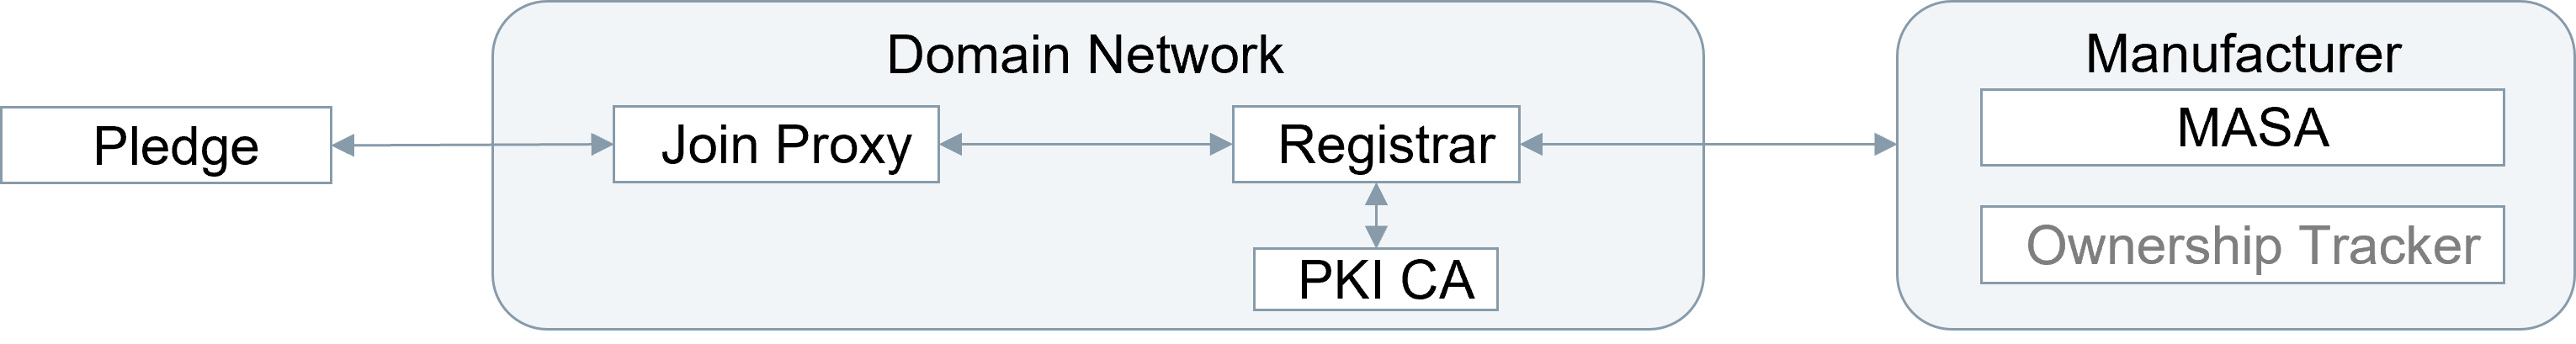
\includegraphics[scale=0.4]{Images/brski-overview.png}
	\caption{BRSKI Architecture.}
	\label{brski-architecture}
\end{figure}

The network domain is the domain of the alleged new owner of the device, i.e the network that is expecting the device to be connected to it. The domain is a network of entities who share a common local trust anchor. 
It incorporates a \gls{pki} to govern the issuance of digital certificates to provide unique digital identifiers for clients and establish end-to-end security. 
\par
A join proxy is another component of the domain. It helps with the discovery of pledges that intend to join the network. In addition, it is responsible for discovering the domain registrar(s) and determining the proxy mechanisms supported by the registrar and utilizing the lowest impact mechanism.
Pledge discovery methods can be classified into passive and active methods. 
GRASP flooding \cite{rfc8990} is a pledge passive discovery method for autonomic networks \cite{kephart2003vision}. It is short for GeneRic Autonomic Signaling Protocol. It is used for signaling between autonomic service agents. GRASP provides discovery, flooding, synchronization, and negotiation functionalities for the technical objectives through respective GRASP messages. Pledge discovery via GRASP multicast flooding is the normative and mandatory method for \gls{brski}.
On the other hand, DNS-based Service Discovery \cite{rfc6763} over Multicast DNS \cite{rfc6762} as well as DHCP \cite{rfc2131} are pledge active discovery methods. They can be used as secondary discovery methods in parallel to GRASP.
Moreover, A proxy provides HTTPS connectivity and forwards messages without examination between a pledge and a registrar in the network, and without interfering with the protocol messages.
\par
A pledge is an unconfigured device attempting to join the network domain. Its goal is to be securely bootstrapped in a zero-touch fashion. To achieve this goal, the pledge establishes a TLS connection with one or more of the domain's registrars through the domain's proxy. It is necessary for the pledge and the registrar to establish mutual authentication. A manufacturer installed \gls{idevid} is used for pledge authentication to the domain's registrar. It is installed during the manufacturing process and includes certificates signed by the manufacturer and unique identifiers that represent the pledge, in addition to, the pledge unique serial number given by the manufacturer. It is recommended that The provided certificates are used for authentication with the registrar and the signing of voucher requests. The unique serial number is used in vouchers and voucher requests to ensure linkability. 
\par
A registrar is an element of the domain that is responsible to carry out the bootstrap process for the pledge. Also, it can be considered as the \gls{ra} for the domain's \gls{pki}. A domain can have one or more registrars which all have to be recognized by the domain proxy. If the pledge is capable to concurrently connect to multiple registrars, it is advisable to do so as this protects against a malicious proxy attempting a \gls{dos} attack like Slowloris.
\par
A manufacturer is the entity that produced the device and set up its initial configuration (IDevID). It provides two distinct services: the \gls{masa} service and ownership tracking and validation.
MASA can be a third party service that signs the vouchers issued for the bootstrapping process. It is also responsible for providing a repository for audit-log information of bootstrapping events. The service is contacted each time a pledge performs a zero-touch bootstrap in an attempt to enroll into a domain. It takes the decision whether or not issue the voucher according to the MASA policy. Voucher issuance could be done blindly at the lowest security level or it could be tightly bound to the sales channel that verifies the actual ownership of the domain. Hence, the manufacturer can provide protection against stolen devices or illegitimate resale of devices by declining voucher issuance to the suspected pledge.
\par
Ownership tracking and validation is an optional manufacturer service. It is supposed to log all claim attempts and to know which device is owned by which domain and provide such information to registrars.  A verified log entry indicates that the pledge was issued a voucher as a result of positive verification of ownership.